\chapter{Aprendizado de regras de transição}

Nas seções seguintes mostraremos resultados da capacidade de autômatos celulares reproduzirem padrões de estruturas secundárias a partir da sequência de aminoácidos e da utilização do EDA para buscar regras de transição. Inicialmente, discutiremos os autômatos celulares e as diferentes opções de estados utilizados. Em seguida, discutiremos os resultados da otimização das regras de transição utilizando um EDA distribuído.  

%Nas seções de resultados a seguir mostraremos a capacidade do EDA em gerar um conjunto de regras de transição  para o autômato celular que permitiu a construção de um preditor de estruturas secundárias capaz de identificar a mudança de poucos aminoácidos na sequencia em contraste com grandes modificações das estruturas secundárias em proteínas camaleônicas. Também, ....

\section{Autômato celular}

Os modelos de autômatos celulares foram testados, até o momento,  no conjunto de proteínas com alta identidade sequencial, mas com grandes diferenças de estrutura secundária, que o torna um problema desafiador. A escolha desse conjunto para os testes dos autômatos celulares baseou-se, também, na facilidade de analisar e visualizar a formação e propagação dos elementos de estruturas secundárias nessas proteínas, pelo fato de serem pequenas.

%A comparação entre os modelos de autômatos celulares foram realizadas primeiramente, e até o momento, apenas no conjunto de proteínas com alta identidade sequencial. A escolha desse conjunto para os testes dos autômatos celulares baseou-se na facilidade de observar e analisar a formação e propagação dos elementos de estruturas secundárias nessas proteínas. É importante ressaltar que ao otimizarmos as regras de transição para este conjunto restrito de proteínas, nosso objetivo é avaliar a capacidade dos modelos propostos de autômatos celulares em recuperar corretamente a estrutura secundária atribuída aos resíduos.   

O modelo idealizado para o autômato celular deveria ter a capacidade de propagar sinais locais ao longo da sequência, e assim, resultar na formação de padrões globais. Tal capacidade está relacionada aos estados que ocorrem durante a evolução do autômato celular, sendo dependentes do número de estados possíveis e também do tamanho da vizinhança utilizada. Como todos os autômatos celulares propostos tem vizinhança 1 (Seção \ref{sssec:ca}), a capacidade de formar e propagar os sinais será dependente apenas dos estados possíveis do autômato celular.

%PSLO Zé essa frase está um pouco confusa: "Como todos os autômatos celulares propostos tem vizinhança 1 (um) por questões de complexidade (ver ref metodos), a capacidade de formar e propagar os sinais será dependente apenas dos estados possíveis do autômato celular."

%Ao otimizarmos as regras apenas para 

Entre os quatro modelos testados, o número de estados para os elementos de estrutura secundária demonstrou relação com a acurácia do modelo. Assim, CAs com estados de elementos de estrutura secundária que conservam mais características dos resíduos mostraram-se mais promissores (Figura \ref{fig:ca_errors}).

\begin{figure}
  \centering
  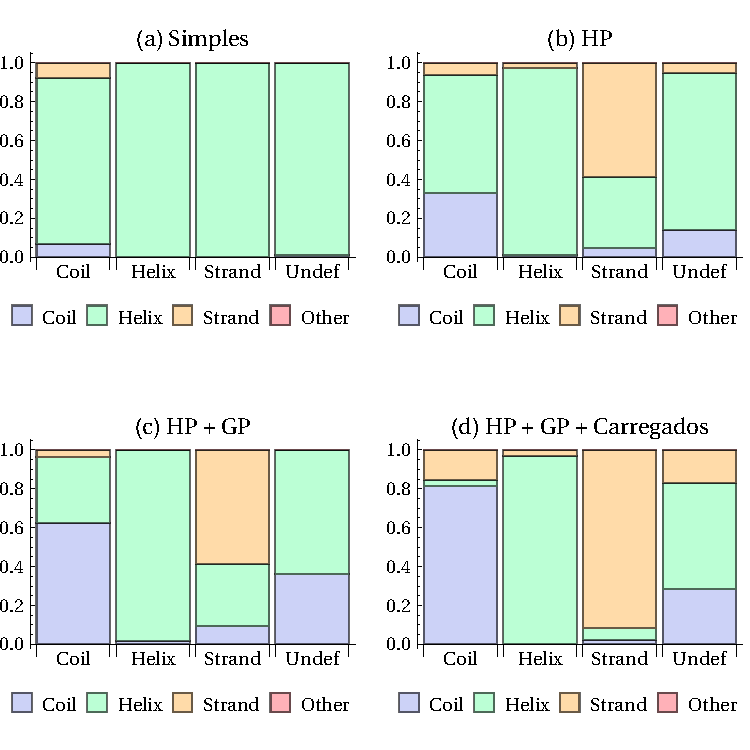
\includegraphics[width=.9\textwidth]{figures/chamel_errors_ca.pdf}
  \caption{Comparação de autômatos celulares com diferentes estados. O gráfico mostra proporção de elementos preditos para cada um dos elementos da estrutura experimental. Em (a) os resultados obtidos por um autômato celular que utiliza apenas 3 estados (H,E,C) para as estruturas secundárias. Em (b) um autômato que apresenta 6 estados, acrescentando as características de hidrofobicidade do resíduo (hidrofóbico/hidrofílico) aos estados de estrutura secundária. Em (c), um autômato celular que apresenta 12 estados após a adição de Gly e Pro como características especias das estruturas secundárias. E por fim, em (d), um autômato celular com 18 estados para as estruturas secundárias onde os estados carregam as características hidrofóbico, hidrofílico, glicina, prolina e resíduos carregados positivamente e negativamente.} 
        \label{fig:ca_errors}
\end{figure}

\begin{figure}
  \centering
  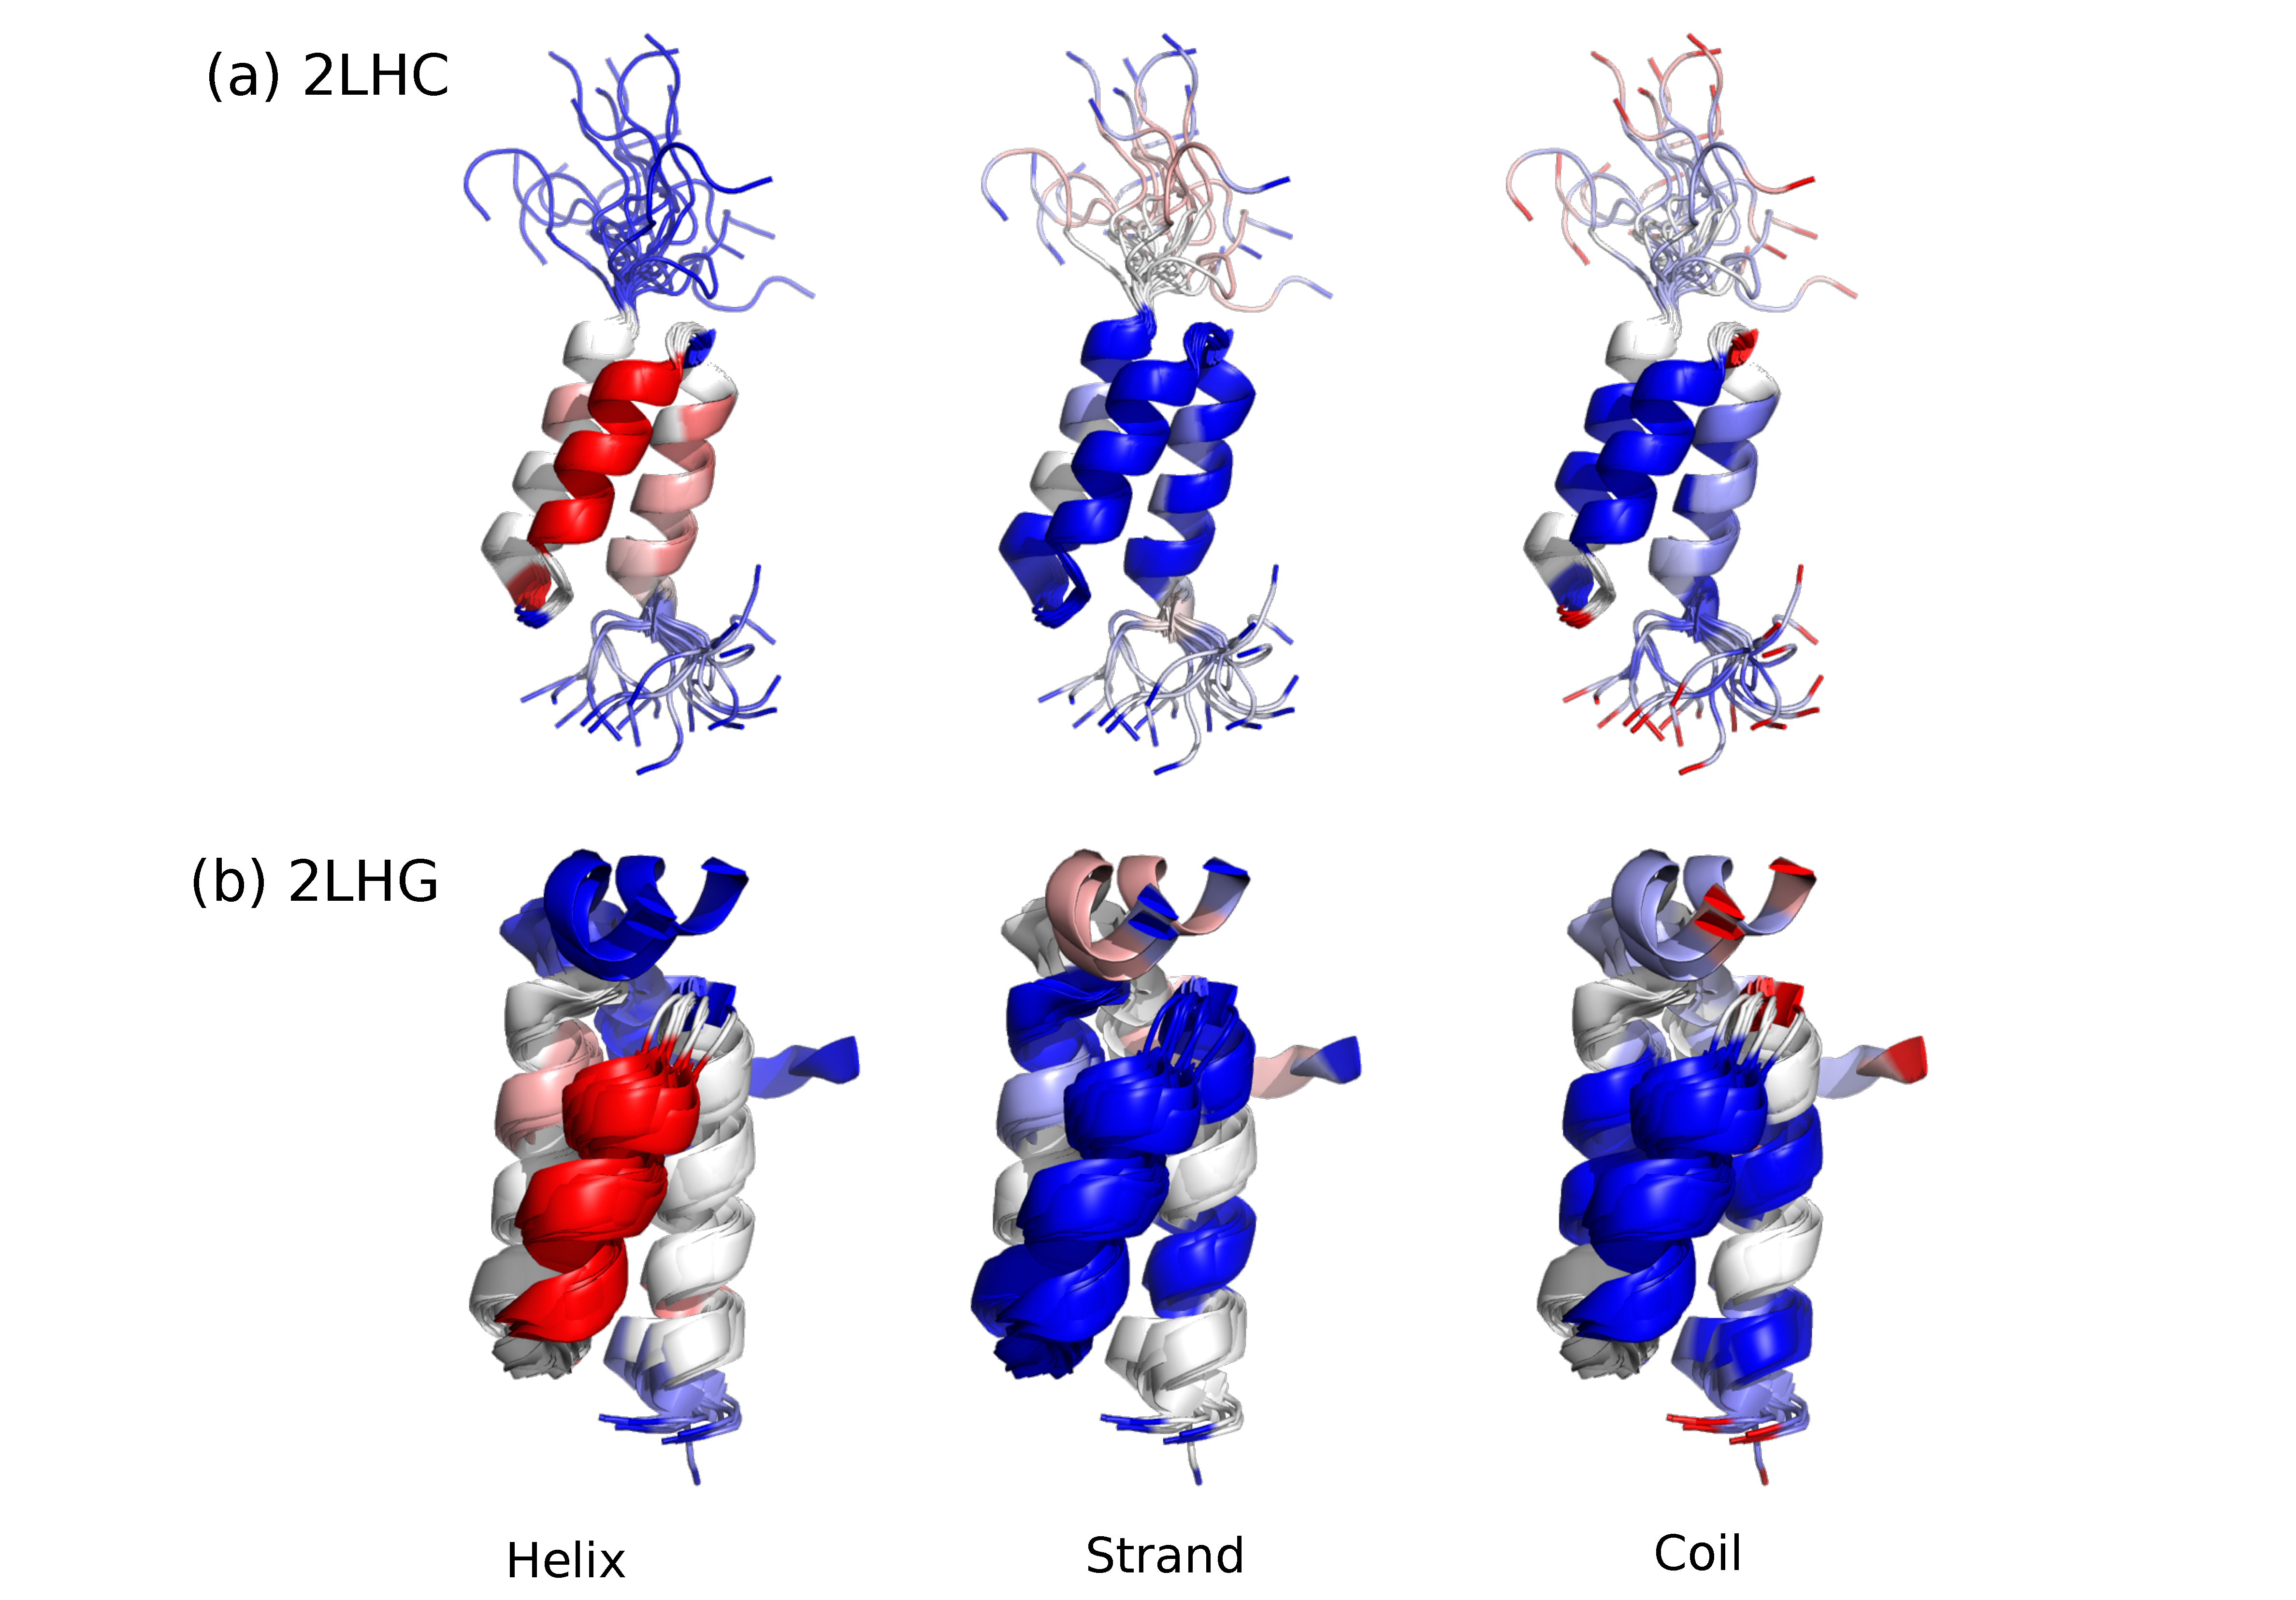
\includegraphics[width=1\textwidth]{figures/camel_2lhc_2lhg.pdf}
  \caption{Modelos estruturais das proteínas Ga98 (PDB ID: 2LHC) e GB98-T25I (PDB ID: 2LHG) que possuem a topologia de feixe de hélices alpha. As cores representam as frequências dos estados durante a evolução do autômato celular num gradiente do vermelho, 100\%, ao azul, 0\%. Cada elemento de estrutura secundária (hélice, fita e coil) corresponde a uma coluna da figura. Notamos que a hélice 2 (intermediária) demonstra alta frequência do estado de hélice no autômato celular após 10000 passos. As outras duas hélices apresentam frequências menores em relação a hélice 2, mas maiores que os outros estados. Entre os resíduos de conexão entre as hélices, aparecem alguns com grande frequência de estados coil. Nas regiões N e C terminais, há uma maior frequência de fitas e coils, em relação à hélices. O autômato celular utilizado possui os estados HP+GP+Carregados.}
        \label{fig:camel_2lhc_2lhg}
\end{figure}

\begin{figure}
  \centering
  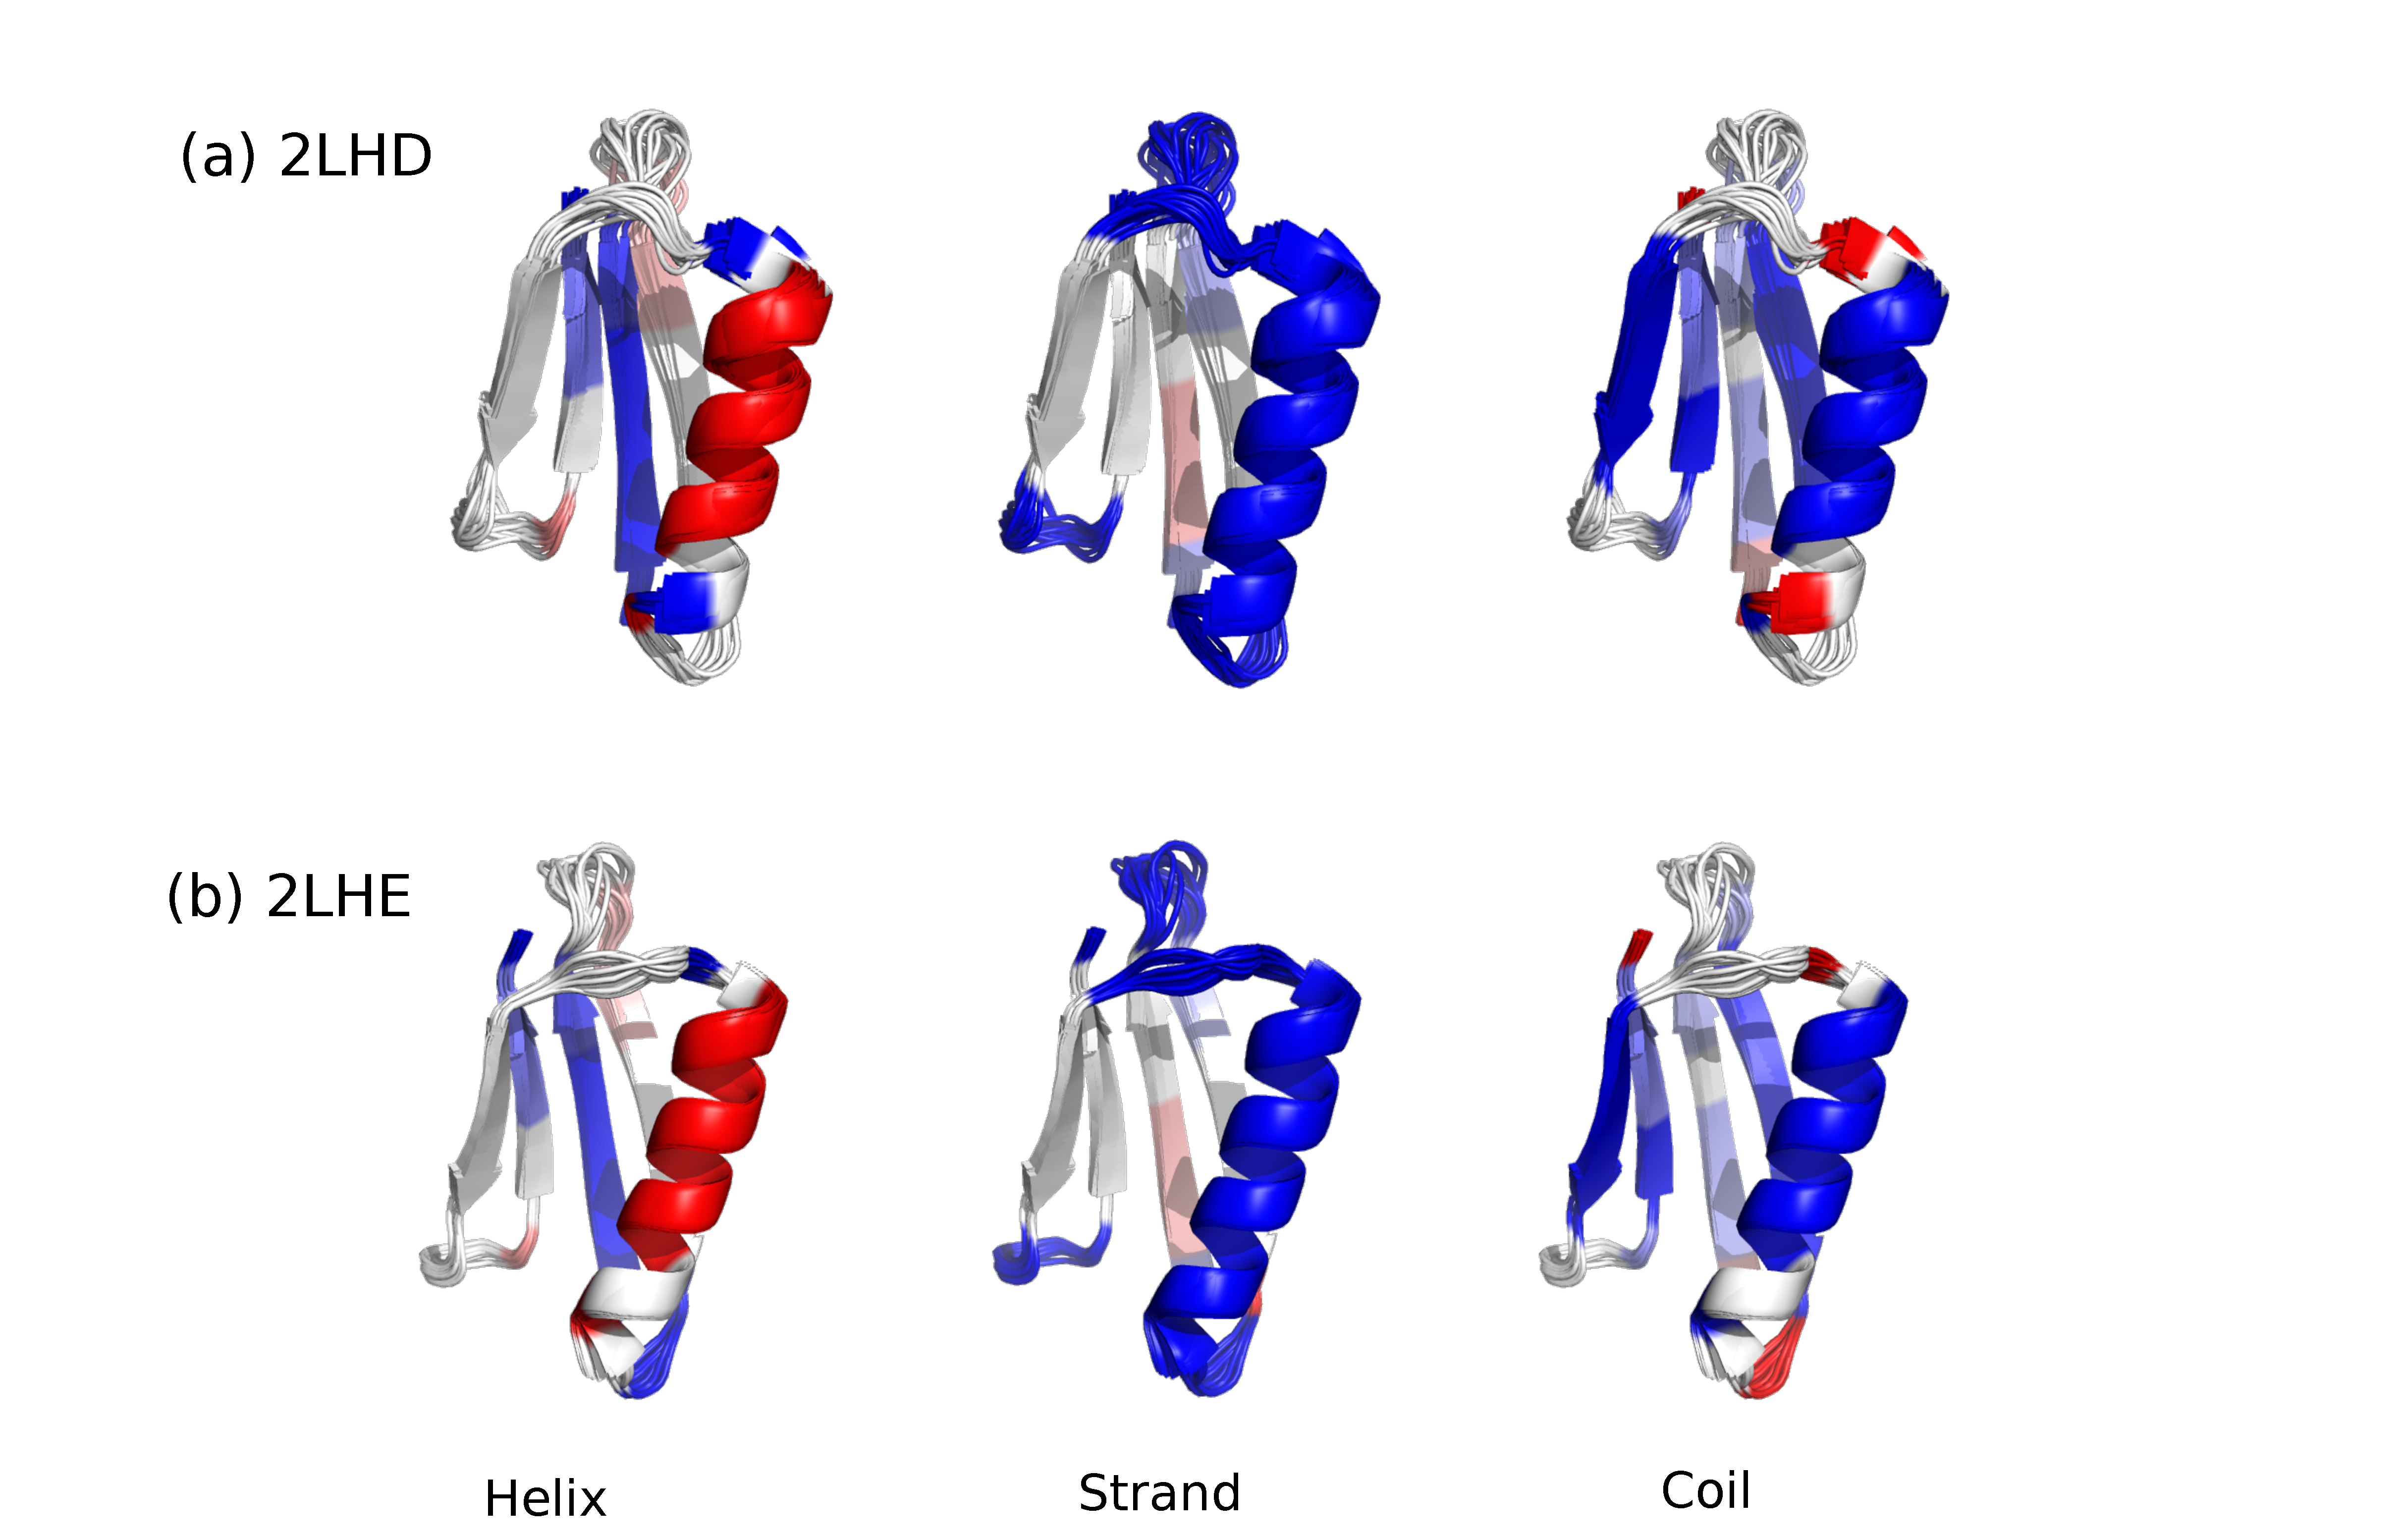
\includegraphics[width=1\textwidth]{figures/camel_2lhd_2lhe.pdf}
  \caption{Modelos estruturais das proteínas GB98 (PDB ID: 2LHD) e GB98-T25I,L20A (PDB ID: 2LHE) que apresentam a topologia de 4 fitas beta e hélice alpha. As cores representam as frequências dos estados durante a evolução do autômato celular num gradiente do vermelho, 100\%, ao azul, 0\%. Cada elemento de estrutura secundária (hélice, fita e coil) corresponde a uma coluna da figura. Notamos que a hélice demonstra alta frequência do estado de hélice no autômato celular após 10000 passos. As fitas apresentam uma frequência tanto estados de hélices como de fitas, exceto a fita 1 que apresenta baixa frequência de hélices e maior frequência de fitas. A regiões de conexão entre as fitas e da hélice com as fitas apresentam maior frequência de coils. O autômato celular utilizado possui os estados HP+GP+Carregados.}
        \label{fig:camel_2lhd_2lhe}
\end{figure}


\section{Análise do desempenho do EDA implementado}

O aprendizado das regras realizado através de um algoritmo de EDA distribuído demonstrou-se eficiente dado a complexidade do problema. Utilizando sete nós (448 núcleos) no cluster de computação de alto desempenho EMU-2 (adquirido pelo "Programa de Equipamento  Multiusuário da FAPESP-2009", 2009/53853-5, localizado no Centro Internacional de Pesquisa e Ensino do Hospital A. C. Camargo em  São Paulo) foi possível evoluir o EDA por 1000 gerações com 10000 indivíduos em pouco menos de duas semanas.

Cada nó de trabalho apresentou um uso de memória de 75\% (48 GB), e manteve o processamento próximo a 100\% por núcleo (1.6 GHz). O mecanismo de comunicação por RPC entre o nó mestre e os nós de trabalho não sobrecarregou a rede (1Gbs). Isso nos permite concluir que o algoritmo é escalável em clusters com maior número de nós e processadores de maior desempenho.

A opção por realizar o torneio entre soluções candidatas nos nós de trabalho, permite apenas a opção de realizar o torneio entre as k últimas soluções geradas no próprio nó. Consequentemente, as k-1 soluções perdedoras são descartadas, havendo portanto, a remoção das soluções perdedoras em cada torneio. 

Usualmente, o método de seleção por torneio utilizado em algoritmos genéticos não distribuídos acumula as solução candidatas até atingir o tamanho máximo populacional, quando então, é realizado o torneio. Isso permite que o torneio seja feito sem a eliminação dos perdedores, possibilitando que a seleção destes ocorram em outros combates.

Entretanto, no EDA distribuído, para aplicarmos um torneio sem eliminação dos perdedores seria necessário:

\begin{enumerate}
	\item o envio de todas as soluções candidatas para o nó mestre, o que resultaria em maior consumo de rede;
	\item o acúmulo de todas as soluções candidatas até atingir o tamanho máximo da população, gerando uma limitação da memória disponível;
	\item a espera até a realização do torneio para iniciar o cálculo das probabilidades, resultando no aumento do tempo ocioso nos nós de trabalho igual ao intervalo de tempo do envio da última solução até a finalização do cálculo das probabilidades.
\end{enumerate} 

A escolha em realizar o torneio nos nós de trabalho demonstrou ser escalável, manter a variabilidade das soluções candidatas ao longo da evolução e convergência (Figura \ref{fig:evo_eda}).

\begin{figure}
  \centering
  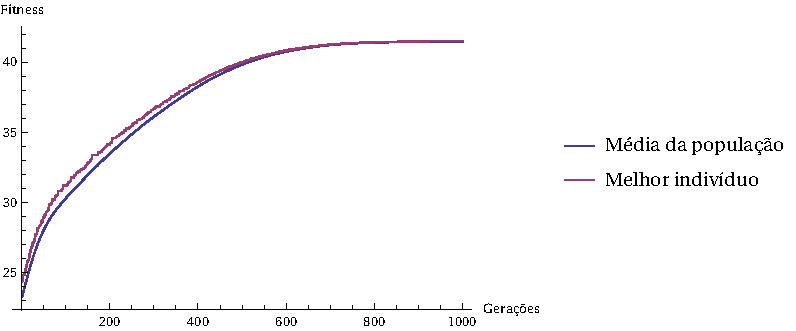
\includegraphics[width=1\textwidth]{figures/evo_Eda.pdf}
  \caption{Gráfico que representa o fitness médio da população de regras candidatas e da melhor regra ao longo de 1000 gerações do EDA.}
        \label{fig:evo_eda}
\end{figure}

\subsection{Deriva genética}

A evolução do EDA por 1000 gerações com torneio de dois (k=2) e população de 10000 indivíduos, demonstrou sinais de deriva genética a partir de 564 gerações. Tais sinais podem ser detectados observando-se as probabilidades dos 38 elementos de regra que não ocorrem no conjunto de proteínas. Esses elementos são do tipo [\#][\textit{x}][\#].

O elementos [\#][\textit{x}][\#], onde o \textit{x} correponde a qualquer estado exceto [\#], não apresentam probabilidade fixa, mas também, por estar ausente nas proteínas, não sofrem pressão seletiva. Logo, suas variações são aleatórias.

Na geração 564 um desses 38 elementos apresentou probabilidade zero ($p=0$), de transitar para um dos quatro estados possíveis, indicando a eliminação de um gene da população por deriva genética. Ao final das 1000 gerações 11 dos 38 elementos apresentavam probabilidade zero para uma das transições (Figura \ref{fig:deriva_genetica}).

%PSLO Zé vc pode trabalhar um pouco mais no texto dessa seção. Eu pelo menos não achei as conclusões muito óbvias

\begin{figure}
  \centering
  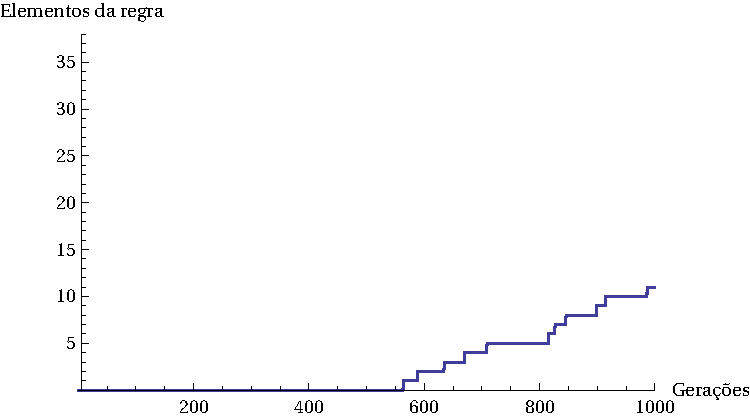
\includegraphics[width=1\textwidth]{figures/deriva_genetica.pdf}
  \caption{Gráfico que indica efeitos de deriva genética através da amostragem de 38 elementos que não sofrem pressão seletiva proveniente do fitness. Na geração 564, um desses elementos apresentou probabilidade igual a zero para uma das transições. Ao final das 1000 gerações, 11 elementos apresentam probabilidade zero para ao menos um dos estados.}
        \label{fig:deriva_genetica}
\end{figure}

% PSLO Zé vamos tentar usar uma tradução para fitness. Senão me engano no capítulo 5 sugeri função de pontuação dos individuos


\subsection{Função de fitness}

A simplicidade da equação de fitness (Equação \ref{eq:fitness}) demonstrou problemas que acreditamos serem solucionáveis na continuação deste trabalho. Um desses problemas é ocasionado pelo desbalanceamento dos dados de treinamento (Figura \ref{fig:occ_ss}). 

\begin{figure}
  \centering
  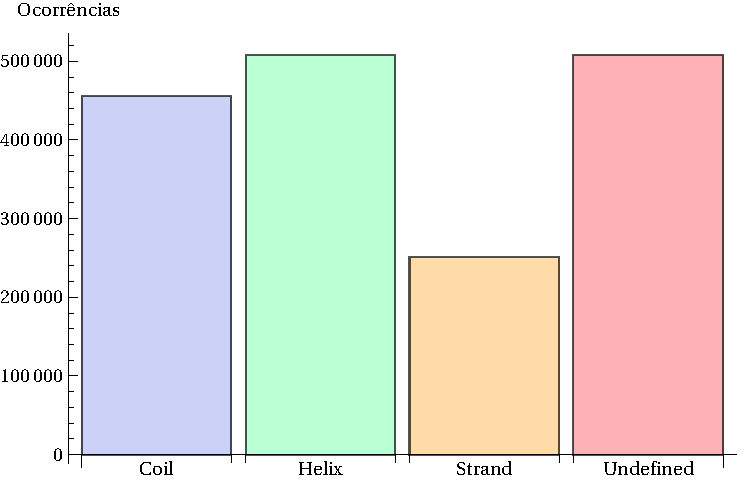
\includegraphics[width=0.9\textwidth]{figures/occ_ss.pdf}
  \caption{Desbalanceamento dos elementos de estrutura secundária no conjunto de dados.}
        \label{fig:occ_ss}
\end{figure}

Os resultados obtidos indicam uma maior acurácia para os elementos de estrutura secundária mais frequentes no conjunto de treinamento. Esse é um problema recorrente no aprendizado com classes desbalanceadas e costuma ser tratado na função de fitness (Figura \ref{fig:q3}), por exemplo, com funções que fazem uma média da acurácia por classes. As alterações na função de fitness para tratar este problema são preferiveis em relação à modificações no conjunto de dados para equibrar as classes, uma vez que modificações no conjunto de dados envolveriam a retirada de informação de classes mais frequentes ou a duplicação de informação das classes menos frequentes, ambas produzindo consequências distorcivas na informação presente no conjunto de treinamento.

%\begin{figure}
%  \centering
%  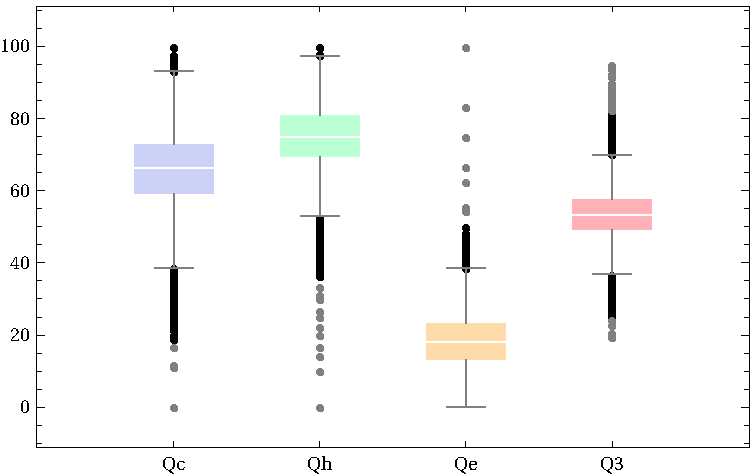
\includegraphics[width=0.9\textwidth]{figures/q3.pdf}
%  \caption{q3}
%        \label{fig:q3}
%\end{figure}

% Avaliamos também se havia alguma relação aparente dos elementos preditos com os ângulos phi e psi do resíduos, o que poderia justificar parcilamente  erros nos elementos preditos. Entretanto, aparentemente não existe tal relação (figuras).



% Roc curve

%Outra modificação possível na função de fitness seria buscar a maximização da frequência dos estados durante a evolução do autômato.  

\subsection{Fatores que influenciam no método de seleção do EDA}

As número de ocorrências de trincas de aminoácidos no conjunto de proteínas apresentou grande variação (Figura \ref{fig:histograma_occ}). Para avaliar a influência dessa variação no EDA nós procuramos por correlações entre fatores que poderiam influenciar na seleção.

\begin{figure}
  \centering
  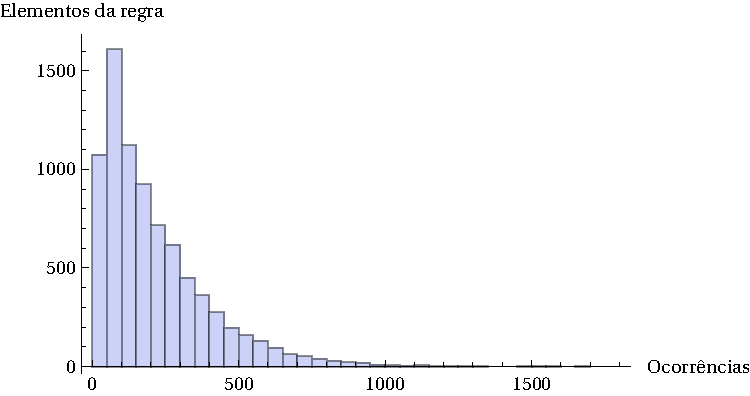
\includegraphics[width=1\textwidth]{figures/histograma_occ.pdf}
  \caption{Histograma de ocorrencia das trincas}
        \label{fig:histograma_occ}
\end{figure}

\begin{table}
\begin{tabular}{cc}
\toprule
\tableheadline{Trinca} & \tableheadline{Frequência}\\
\midrule
CCW & 2\\
CMW & 2\\
WMC & 2\\
WPC & 3\\
WCW & 3\\
CHW & 4\\
\bottomrule
\end{tabular}
\quad
\begin{tabular}{cc}
\toprule
\tableheadline{Trinca} & \tableheadline{Frequência}\\
\midrule
EAL & 1316\\
LAA & 1478\\
AAL & 1534\\
ALA & 1563\\
AAA & 1682\\
HHH & 6143\\
\bottomrule
\end{tabular}
\caption{Trincas de aminoácidos menos (à esquerda) e mais (à direita) frequentes no conjunto de treinamento.}
\end{table}



A figura \ref{fig:probG999_occXprob} representa a distribuição das probabilidades máximas e mínimas dos elementos da regra em relação a frequência de ocorrência das trincas de aminoácidos no conjunto. O gráfico e o valor de correlação (Spearman = 0.09) entre as probabilidades e a frequência de ocorrência das trincas,  indica não haver uma grande influência da frequência das trincas durante a seleção. Essa influência também não foi encontrada durante a evolução do EDA (Anexo).  

%incluir as figuras do anexo

\begin{figure}
  \centering
  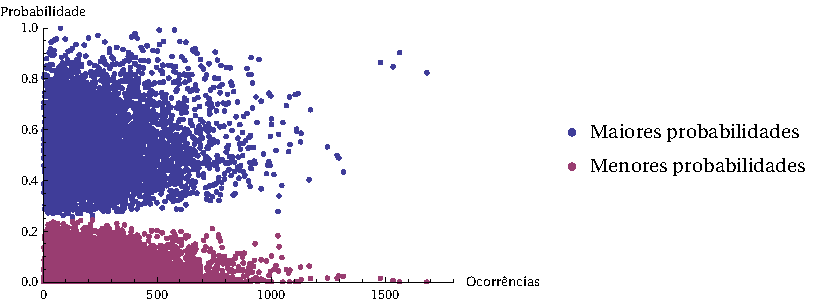
\includegraphics[width=1\textwidth]{figures/probG999_occXprob.pdf}
  \caption{Probabilidades máximas e mínimas dos elementos da regra de transição em relação ao número de ocorrência das trincas de aminoácidos.}
        \label{fig:probG999_occXprob}
\end{figure}


Outros fatores que poderiam influenciar a evolução do EDA seriam: \textit{(1)} a probabilidade da trinca ser observada em uma determinada estrutura secundária; \textit{(2)} o número de ocorrências da trinca em determinada estrutura secundária; \textit{(3)} a taxa de acertos por trincas para determinada estrutura secundária. 

%ta estranho essa parte    

As probabilidades de transição dos elementos da regra, não apresentam aparente relação com as proporções encontradas para cada estrutura secundária nas trincas (Figura \ref{fig:relacao_prob_propss}). Assim como não apresentaram relação com a frequência de ocorrências de determinada estrutura para uma trinca e com a proporção de trincas corretamente classificadas por estrutura secundária. Essas duas últimas relações não eram mesmo esperadas (Anexo Figuras H E C e figuras H E C). Contudo, foi interessante observar que a primeira relação aparentemente não ocorria.

%PSLO Para uma taxa de acertos maior eu deveria esperar que acontece uma correlação alta entre a probabilidade gerada pelo EDA para uma dada regra para uma certa estrutura secundaria específica.   

\begin{figure}
  \centering
  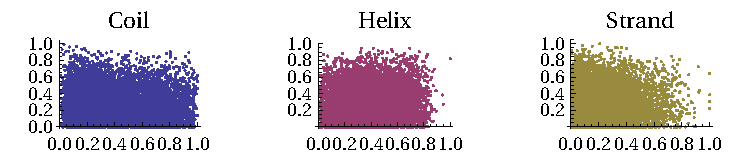
\includegraphics[width=1\textwidth]{figures/relacao_prob_propss.pdf}
  \caption{Relação entre a proporção de uma trinca de aminoácidos em determinada estrutura secundária e a probabilidade resultante da otimização utilizando EDA.}
        \label{fig:relacao_prob_propss}
\end{figure}

A ausência da primeira relação pode indicar que as probabilidades de transição dos demais elementos da regra e sua aplicação ao longo da evolução do CA estão propagando as probabilidades e sofrendo influência da vizinhança na busca de produzir estruturas secundárias mais próximas as reais. 

Entretanto, observamos uma relação entre a proporção de elementos de estruturas secundárias para um trinca e a proporção de acertos da trinca para a mesma estrutura secundária. Acreditamos que isso seja um indício que o aprendizado, ou otimização da regra, precisa ser melhorado para que elementos de estruturas secundárias menos comuns a determinadas trincas possam ser corretamente preditos (Figura \ref{fig:prop_acerto} e Tabela \ref{tab:corr_acertos}).  

\begin{figure}
  \centering
  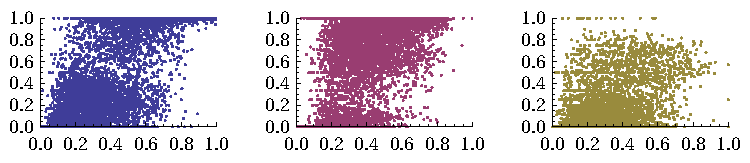
\includegraphics[width=1\textwidth]{figures/prop_acerto.pdf}
  \caption{Relação proporção de acertos x probabilidade EDA}
        \label{fig:prop_acerto}
\end{figure}

Há também uma relação menos influente entre o número de ocorrências de uma determinada estrutura secundária nas trincas e a proporção de acertos dessa trinca para a mesma estrutura secundária (Figura \ref{fig:occ_acerto} e Tabela \ref{tab:corr_acertos}).

\begin{figure}
  \centering
  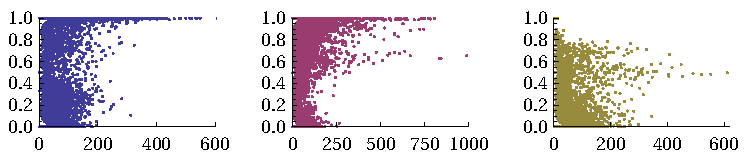
\includegraphics[width=1\textwidth]{figures/occ_acerto.pdf}
  \caption{Relação ocorrencias das ss por trincas x probabilidade EDA}
        \label{fig:occ_acerto}
\end{figure}

\begin{table}
    \myfloatalign
    \label{tab:corr_acertos}
  \begin{tabularx}{\textwidth}{Xlll} \toprule
    \tableheadline{Correlação}   & \tableheadline{coil}   & \tableheadline{hélices}  & \tableheadline{fitas} \\ 
    \midrule
     Proporção das trincas  & 0,75 & 0,60   & 0,60   \\
    Ocorrências das trincas  & 0,60 & 0,24   & 0,38  \\
    %autem vulputate ex & parola & romanic \\
    %usu mucius iisque & studio & sanctificatef \\
    \bottomrule
  \end{tabularx}
  \caption{Correlação (Spearman) entre a proporção de acertos na predição e: (1) proporção das trincas nas estruturas secundárias, (2) número de ocorrências das trincas nas estruturas secundárias}
\end{table}

Ambas as relações encontradas eram esperadas pois indicam uma tendência do método a privilegiar o aprendizado, ou otimização, de elementos capazes de influenciar com maior intensidade a função de fitness. Isso mostra a importância de manter um variabilidade alta na população e reduzir efeitos de deriva genética para que a otimização escape de mínimos locais e consiga aprender, também, as probabilidades para trincas menos frequentes nas proteínas e/ou com proporções pequenas para determinadas estruturas secundárias.

%\chapter{Aprendizado das regras gerais}




% \section{contagem de aa}
% CCW      2
% CMW      2
% WMC      2
% WPC      3
% WCW      3
% CHW      4
% MWC      4
% CCC      4
% CMC      4
% WCC      4
% CWW      4
% WWM      5
% MCW      5
% CWC      5
% MWM      6
% CCM      6
% MWH      6
% CWH      6
% FWC      6
% QCC      6
% QCW      6
% WWW      6
% WCH      7
% CMM      7
% YCW      7
% WCM      7
% CIW      7
% HWC      7
% CQW      7
% CYW      8
% ..     ...
% AAE   1000
% LKE   1001
% AEA   1011
% EAA   1021
% AGA   1029
% AGL   1032
% AAV   1034
% AEL   1046
% ELA   1051
% EEL   1066
% ALG   1076
% LGL   1080
% LAG   1082
% VAA   1105
% ALE   1111
% LEA   1111
% AVA   1118
% ELL   1129
% LAL   1131
% LLE   1166
% LAE   1172
% AAG   1246
% ALL   1289
% LLA   1296
% EAL   1316
% LAA   1478
% AAL   1534
% ALA   1563
% AAA   1682
% HHH   6143